\documentclass{report}

\usepackage{graphicx}
\usepackage{subcaption}

\begin{document}

\title{PicnicHealth Interview Question}
\author{Richard Hauser}
\date{7/14/2019}
\maketitle

	I don't want to go out bike riding when the weather is poor. If I feel like way, then clearly everyone else must feel the same. This purely personal opinion can be quantified using the weather and bike share data given in the question prompt. From a basic analysis of the data we can see that as the weather gets colder and/or precipitation occurs, fewer people are using bike shares. We can also see that the behavior changes mostly with the “customers”, people who use the service irregularly compared to “subscribers”.

	First, let us take a look at the entire population to get a feel for what we are looking at. We have a lot of temperature variables, precipitation, and bike share behavior. Rather than overload ourselves with graphs to look at, our focus here will be on five primary variables, average daily temperature, daily precipitation, total ride time, average ride time, and daily riders. Here in Figure \ref{fig:AllCorr} we have used Kendall's tau coefficient to find the correlation between these different variables. The key takeaways here are that warmer temperatures result in more riders and higher precipitation results in fewer riders. 

\begin{figure}[h!]
	\begin{subfigure}[b]{0.5\linewidth}
		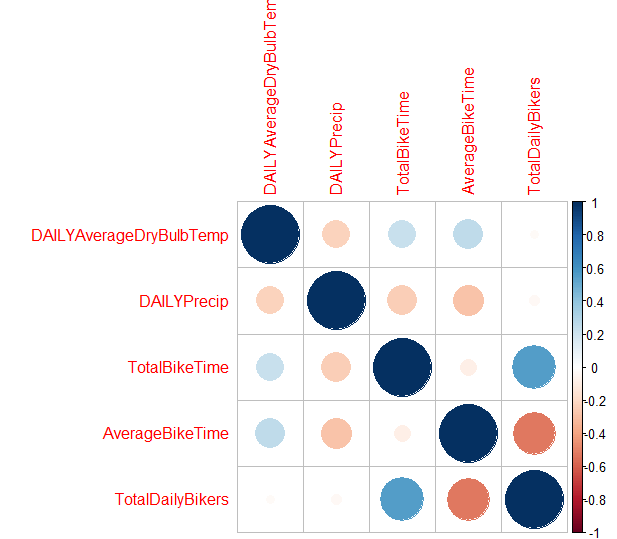
\includegraphics[width=\linewidth]{Corrrelation.png}
	\end{subfigure}
	\begin{subfigure}[b]{0.5\linewidth}
		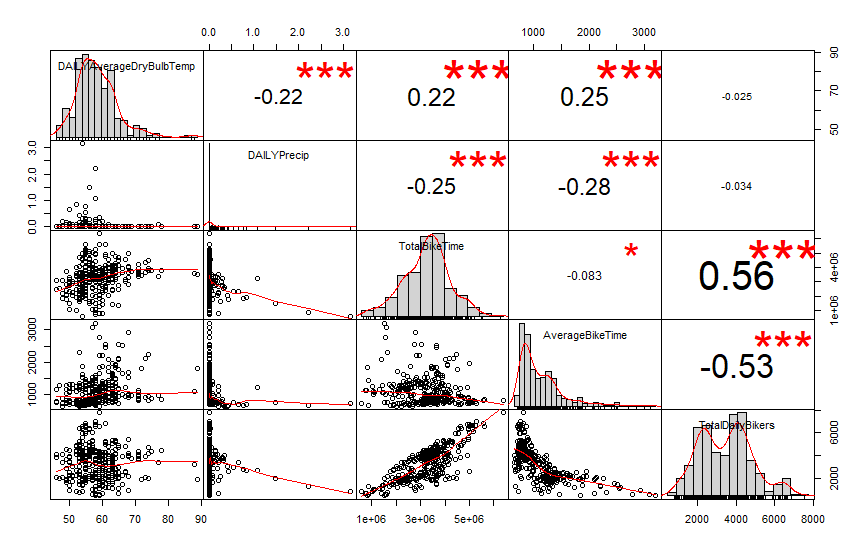
\includegraphics[width=\linewidth]{CorrScatter.png}
	\end{subfigure}
	\caption{Correlation Between Weather and Bike Share}
	\label{fig:AllCorr}
\end{figure}


	There are a few caveats here that deserve acknowledgment and additional refinement in our model. First, precipitation is at 0 nearly 84\% of the measured days. This skews the distribution heavily towards no rain, making the precipitation look like a zero-inflated Poisson distribution. While this does not invalidate the results of the correlation, it does suggest a more refined approach would take into account this skew. Secondly, we are assuming there is only one class of biker. If there are multiple reasons people use bike share, their behavior in relation to the weather may change.

	When we take a look at the usage behavior in Figure \ref{fig:AllHeatmap} we see a clear message. There is heavy usage during commuting hours. If we can extract the commuters from the picture, we may be able to use different classifications of bikers to gain more insight into behavior.

\begin{figure}[h!]
	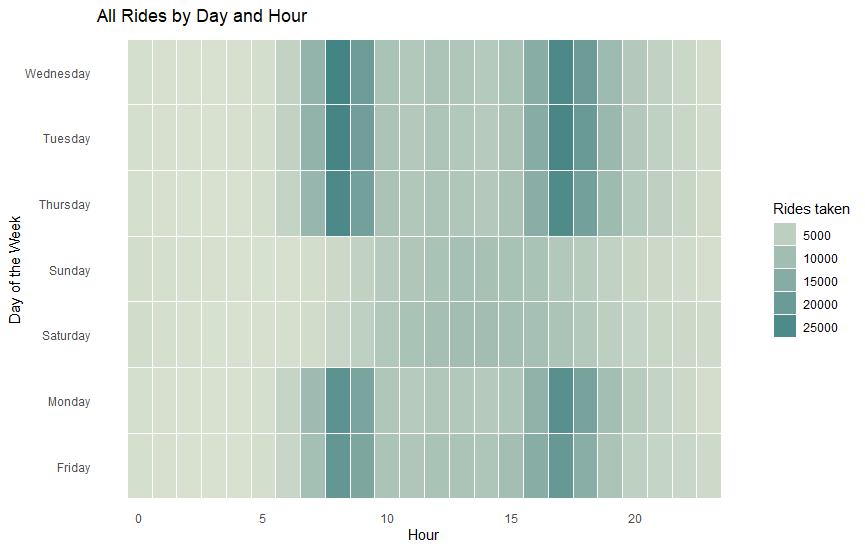
\includegraphics[width=\linewidth]{HeatmapAll.png}
	\caption{Weekly Bike Share Behavior}
	\label{fig:AllHeatmap}
\end{figure}


	The bike share data provides us with a user\_type column consisting of “customers” and “subscribers”. If we compare the usage rates of these two populations using the heatmaps in Figure \ref{fig:SplitHeatmap}, we can see they are quite different. The subscribers appear to primarily be users who regularly use the bike shares for commuting. This is evidenced by the high usage rates on weekdays around 8 AM and 5 PM. If we compare the heat map to customers, while we see some increased activity around commuting times, they most heavily use bike shares on the weekends during the day. If this customer population is as I suspect, they are using the bike share for elective or recreational purposes. This population should be the most affected by weather, as they could delay their activity, unlike someone using the bike share for their commute.

\begin{figure}[h!]
	\begin{subfigure}[b]{0.5\linewidth}
		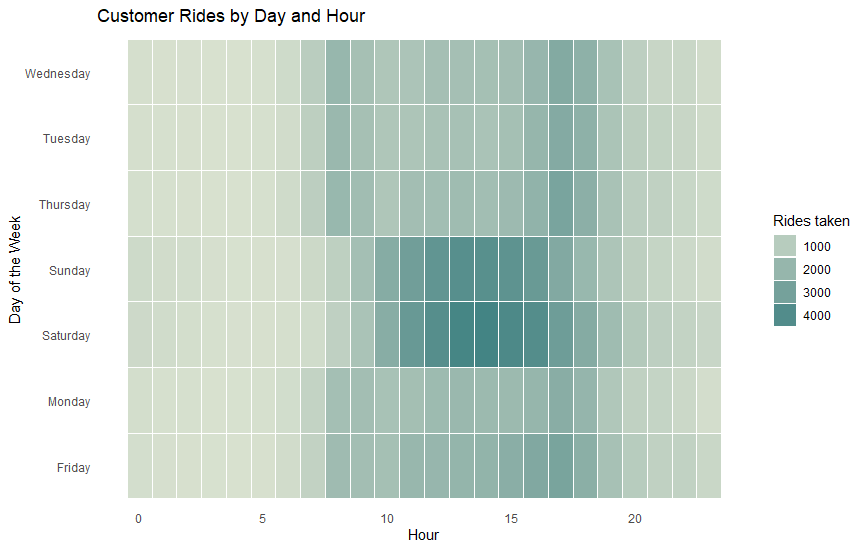
\includegraphics[width=\linewidth]{HeatmapCus.png}
		\caption{Customer}
	\end{subfigure}
	\begin{subfigure}[b]{0.5\linewidth}
		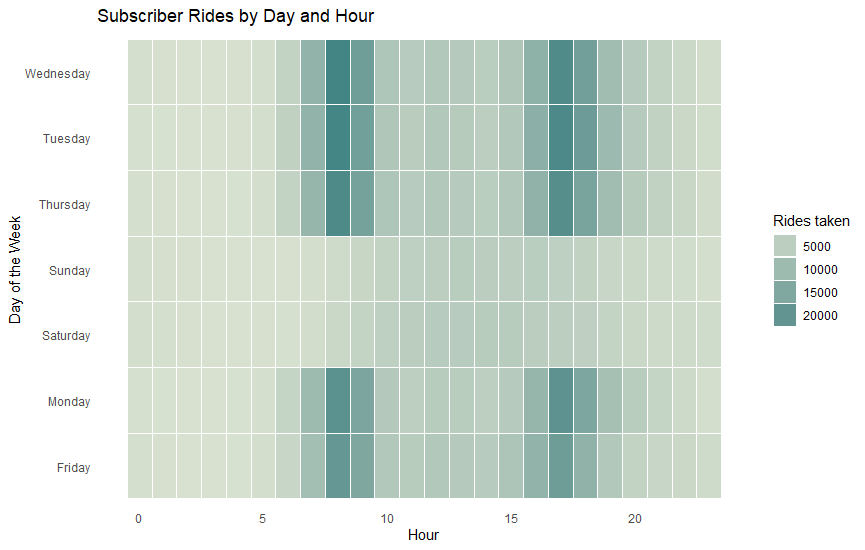
\includegraphics[width=\linewidth]{HeatmapSub.png}
		\caption{Subscriber}
	\end{subfigure}
	\caption{Customer/Subscriber Bike Share Behavior}
	\label{fig:SplitHeatmap}
\end{figure}

	When we compare the correlation between weather and bike share activity after separating the two groups, we find the difference to be quite stark. The scatterplots and correlation coefficients are shown in Figures \ref{fig:CustHis} and \ref{fig:SubHis}. We can see a moderate correlation between the number of bikers going out in poor weather among the customer population. This is what we were expecting to see. The big difference from our whole population sample is when we look at the commuter population. This population does not change their decision to use a bike share according to the weather. There is a relationship between the time a bike is used and the weather, perhaps suggesting regardless of the population people prefer to bike less in poor weather. It is clear however the two populations have very different behaviors, supporting our hypothesis that weather does not change the decision for commuters to use a bike share, whereas customers do.

\begin{figure}[h!]
	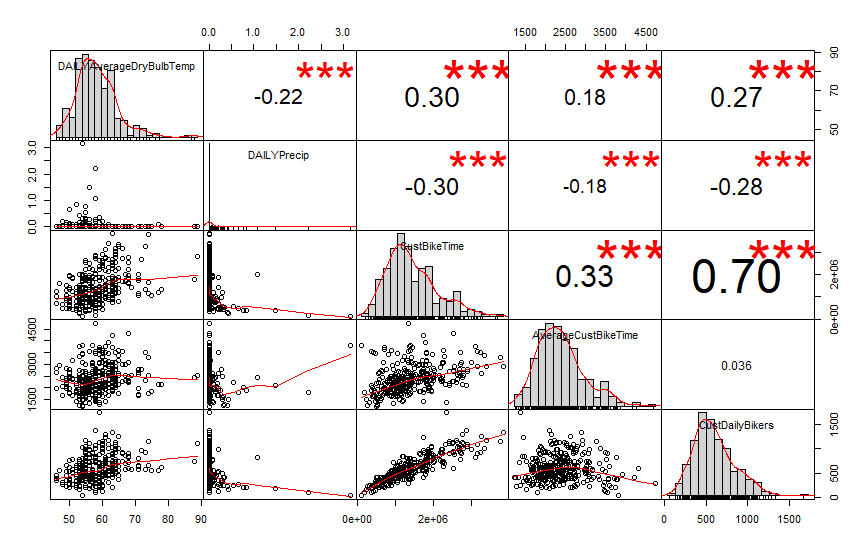
\includegraphics[width=\linewidth]{CorrCust.png}
	\caption{Customer Behavior Histograms}
	\label{fig:CustHis}
\end{figure}
\begin{figure}[h!]
	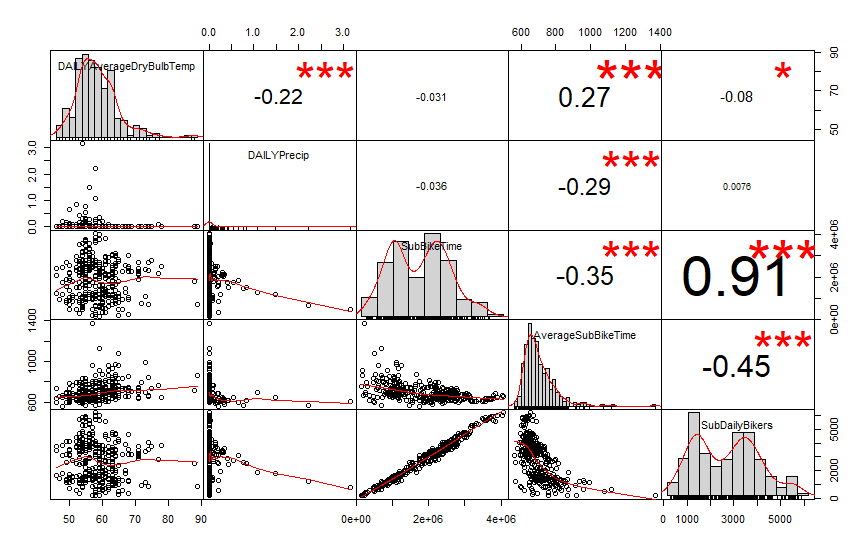
\includegraphics[width=\linewidth]{CorrSub.png}
	\caption{Subscriber Behavior Histograms}
	\label{fig:SubHis}
\end{figure}


	While we have shown that casual bikers are more likely to use bike shares during good weather, there are additional insights that could be gained through additional analysis. We have not looked at the relationship between the day of the week and weather. Poor weather could have a greater effect on the weekends when most users are more likely to use the bike share selectively. Additionally, we have used temperature as a warmer temperature is better for riding, but that is probably not always the case. Activity in relationship to temperature may follow more of a bi-modal distribution, where a sweet spot hits between high and low temperatures. It is hard to judge the high end of the temperature spectrum because it rarely hits a very high temperature in San Francisco. In the end, while there are countless ways to try to improve the analysis, we have shown here that customers are the ones primarily changing bike share habits in response to changes in weather.

\end{document}